As mentioned in section \ref{sec:reqspec}, it is the goal of this project to construct a working prototype. It will include a GUI (graphical user interface) which will guide the user through the system.\\

When the system is installed and the program is run for the first time, it will prompt the user to calibrate. The calibration will consist of finding the table and having the user to identify the balls with mouse clicks. The calibration will only be done once. When the system is calibrated the program will load the calibration configurations every time it starts. Re-calibration will have to be done if the camera or table changes position or if the system is installed in a place where the balls have different colors.\\

For normal use the system will have the options of recording pool games and viewing previously recorded games. The recording will consist of the position of each ball for every change in the game state. The game state is considered to have changed if one of the following occurs:\\ 
\begin{itemize}
	\item The positions of the balls have changed.
	\item When the number of balls have changed.
\end{itemize}

\subsection{Program flow}
The goal is to record the positions of the balls between every change in the game and save this as a state. To do this automatically, the program will have to know when the state has changed and when the game is finished. A state change will only occur when players interact with the table, i.e. they either strike a ball using a cue or move balls manually. Because of this, checking for state changes only has to be done when human interaction has been detected. We define human interaction as the following event:
\begin{itemize}
	\item  A foreign object (que, hand etc.) has been introduced onto the cloth of the pool table and afterwards removed.
\end{itemize}

The system will save a new state if one of the following conditions is fulfilled:

\begin{itemize}
	\item The number of balls has changed
	\item The position of one or more balls has changed
\end{itemize}

These conditions are based on the knowledge that human interaction will introduce a foreign object on the cloth.  An introduction of a foreign object does not necessarily conclude a change in the game state, therefore the newly sampled game state will be compared to the latest saved game state.

The program flowchart can be seen in \ref{fig:program_flowchart}.\\

\begin{figure}[H]
\begin{center}
\leavevmode
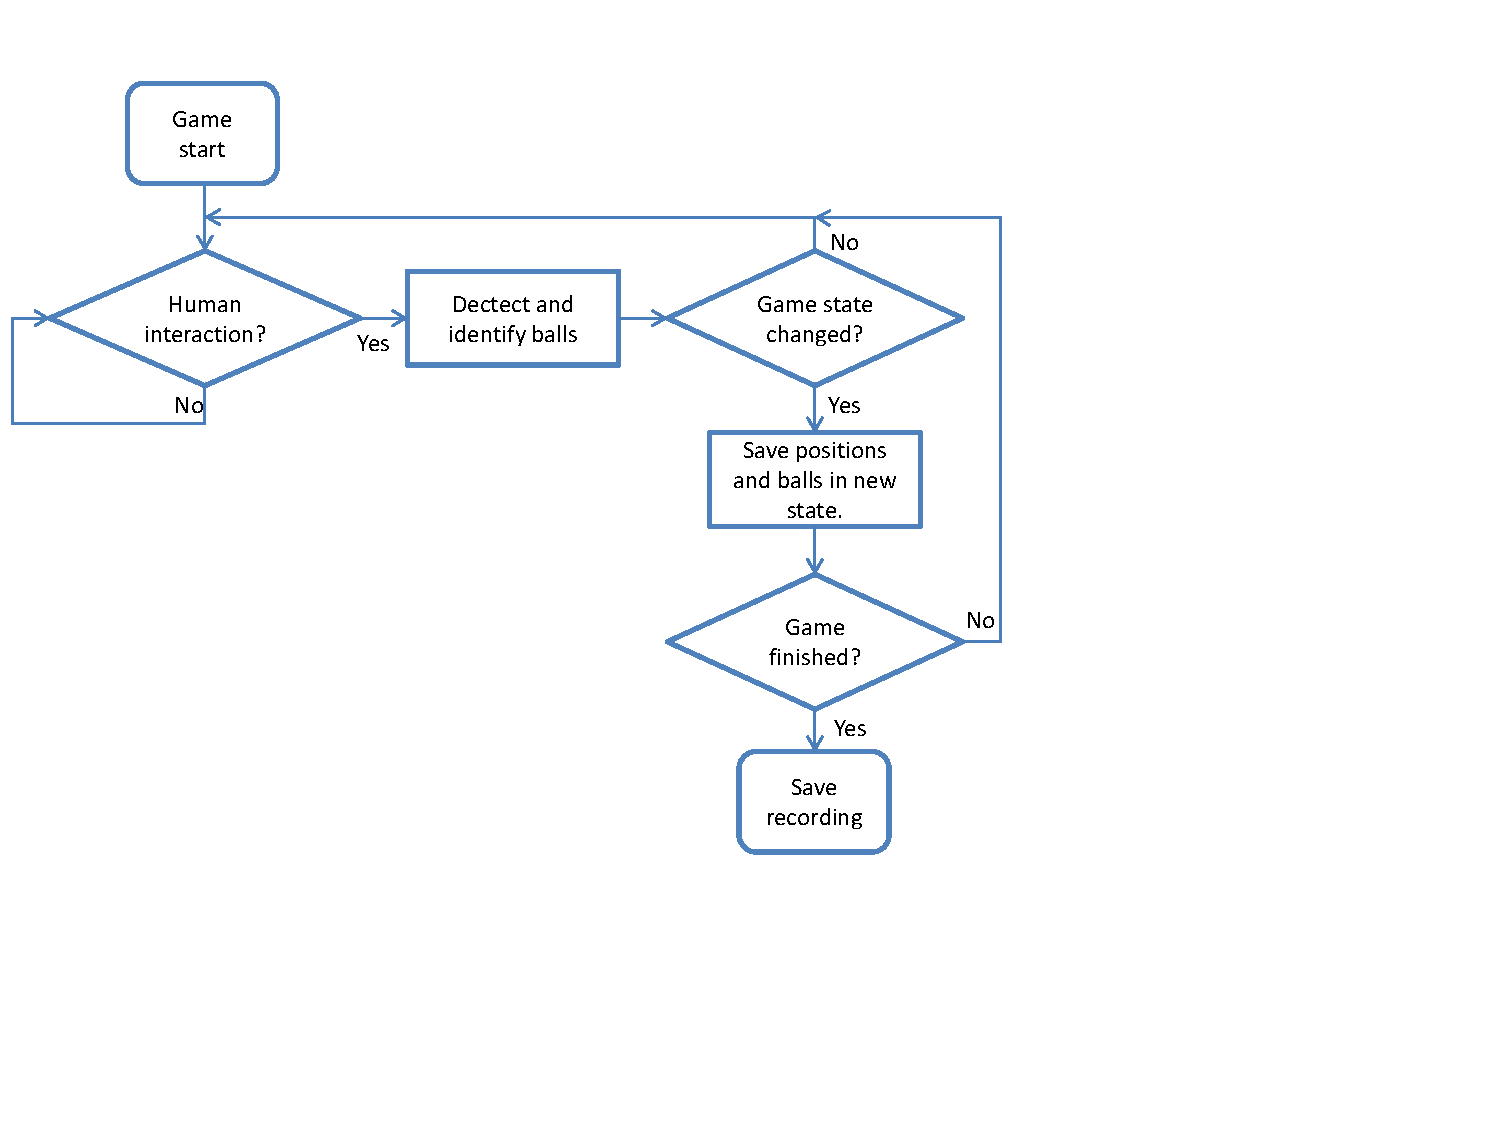
\includegraphics[width=0.8\textwidth]{images/program_flowchart}
\end{center}
\caption{Flowchart of the PoolTracker program while running.}
\label{fig:program_flowchart}
\end{figure}

The game will start when the user decides to do so. The detection of human interaction will be explained in section \ref{sec:shotdetection}. The movement of balls will be explained in section in\ref{sec:shotdetection} based on the balls positions which will be found in section \ref{sec:balls-locate}.

\subsection{Calibration flow}
The calibration have to be done every time the camera changes position or when the system is installed for the first time. The calibration is done to locate table and to train the system with the colors of the balls. The calibration flowchart can be seen in \ref{fig:calib_flowchart}.\\

\begin{figure}[H]
\begin{center}
\leavevmode
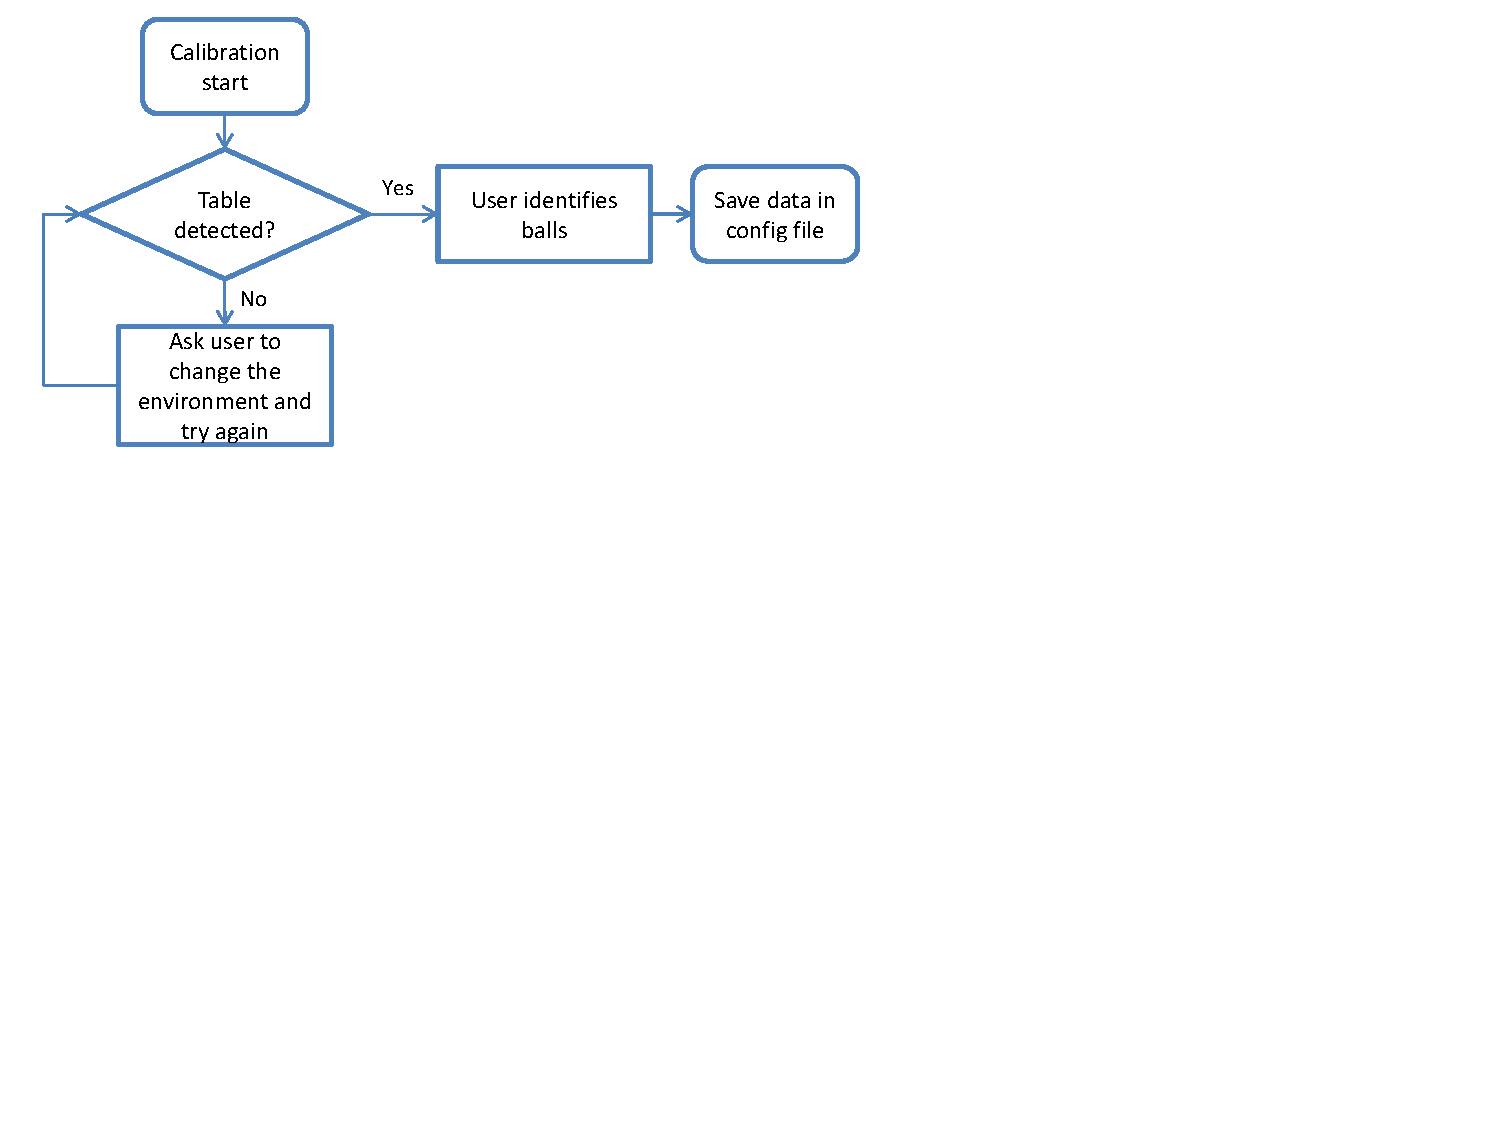
\includegraphics[width=0.8\textwidth]{images/calib_flowchart}
\end{center}
\caption{Flowchart of the PoolTracker program in calibration.}
\label{fig:program_flowchart}
\end{figure}

Table location is explained in \ref{sec:table-locate}. The calibration of balls is explained in\ref{sec:identify-balls}.


